%%
%% Copyright 2007, 2008, 2009 Elsevier Ltd
%%
%% This file is part of the 'Elsarticle Bundle'.
%% ---------------------------------------------
%%
%% It may be distributed under the conditions of the LaTeX Project Public
%% License, either version 1.2 of this license or (at your option) any
%% later version.  The latest version of this license is in
%%    http://www.latex-project.org/lppl.txt
%% and version 1.2 or later is part of all distributions of LaTeX
%% version 1999/12/01 or later.
%%
%% The list of all files belonging to the 'Elsarticle Bundle' is
%% given in the file `manifest.txt'.
%%

%% Template article for Elsevier's document class `elsarticle'
%% with harvard style bibliographic references
%% SP 2008/03/01
%%
%%
%%
%% $Id: elsarticle-template-harv.tex 4 2009-10-24 08:22:58Z rishi $
%%
%%
%%\documentclass[preprint,authoryear,12pt]{elsarticle}

%% Use the option review to obtain double line spacing
\documentclass[authoryear,preprint,review,12pt]{elsarticle}

%% Use the options 1p,twocolumn; 3p; 3p,twocolumn; 5p; or 5p,twocolumn
%% for a journal layout:
%% \documentclass[final,authoryear,1p,times]{elsarticle}
%% \documentclass[final,authoryear,1p,times,twocolumn]{elsarticle}
%% \documentclass[final,authoryear,3p,times]{elsarticle}
%% \documentclass[final,authoryear,3p,times,twocolumn]{elsarticle}
%% \documentclass[final,authoryear,5p,times]{elsarticle}
%% \documentclass[final,authoryear,5p,times,twocolumn]{elsarticle}

%% if you use PostScript figures in your article
%% use the graphics package for simple commands
\usepackage{graphics}
\usepackage{longtable}
\usepackage{url}
%% or use the graphicx package for more complicated commands
%% \usepackage{graphicx}
%% or use the epsfig package if you prefer to use the old commands
%% \usepackage{epsfig}

%% The amssymb package provides various useful mathematical symbols
\usepackage{amssymb}
%% The amsthm package provides extended theorem environments
\usepackage{amsthm}
\usepackage{colortbl}

% For psudo code
\usepackage{amsmath}
\usepackage{algorithm}
\usepackage[noend]{algpseudocode}
\usepackage{setspace}

\makeatletter
\def\BState{\State\hskip-\ALG@thistlm}
\makeatother

%% The lineno packages adds line numbers. Start line numbering with
%% \begin{linenumbers}, end it with \end{linenumbers}. Or switch it on
%% for the whole article with \linenumbers after \end{frontmatter}.
%% \usepackage{lineno}

%% natbib.sty is loaded by default. However, natbib options can be
%% provided with \biboptions{...} command. Following options are
%% valid:

%%   round  -  round parentheses are used (default)
%%   square -  square brackets are used   [option]
%%   curly  -  curly braces are used      {option}
%%   angle  -  angle brackets are used    <option>
%%   semicolon  -  multiple citations separated by semi-colon (default)
%%   colon  - same as semicolon, an earlier confusion
%%   comma  -  separated by comma
%%   authoryear - selects author-year citations (default)
%%   numbers-  selects numerical citations
%%   super  -  numerical citations as superscripts
%%   sort   -  sorts multiple citations according to order in ref. list
%%   sort&compress   -  like sort, but also compresses numerical citations
%%   compress - compresses without sorting
%%   longnamesfirst  -  makes first citation full author list
%%
%% \biboptions{longnamesfirst,comma}

% \biboptions{}

\journal{Expert Systems with Applications}

\newtheorem{definition}{Definition}
\newtheorem{proposition}{Proposition}

\begin{document}

\begin{frontmatter}

%% Title, authors and addresses

%% use the tnoteref command within \title for footnotes;
%% use the tnotetext command for the associated footnote;
%% use the fnref command within \author or \address for footnotes;
%% use the fntext command for the associated footnote;
%% use the corref command within \author for corresponding author footnotes;
%% use the cortext command for the associated footnote;
%% use the ead command for the email address,
%% and the form \ead[url] for the home page:
%%
%% \title{Title\tnoteref{label1}}
%% \tnotetext[label1]{}
%% \author{Name\corref{cor1}\fnref{label2}}
%% \ead{email address}
%% \ead[url]{home page}
%% \fntext[label2]{}
%% \cortext[cor1]{}
%% \address{Address\fnref{label3}}
%% \fntext[label3]{}

\title{Technical Report on a New Fast Hardware Software Platform for Computing Reducts}

%% use optional labels to link authors explicitly to addresses:
%% \author[label1,label2]{<author name>}
%% \address[label1]{<address>}
%% \address[label2]{<address>}


\address{Computer Science Department}
\address{National Institute for Astrophysics, Optics and Electronics}
\address{Sta. Ma. Tonanzintla, Puebla, 72840, Mexico}

\begin{abstract}
	This paper deals with the problem of computing all reducts of an information system. Reducts are useful for attribute reduction in classification problems and data size reduction. Unfortunately, finding the all reducts of an information system has exponential complexity regarding the number of attributes. Several algorithms have been reported to overcome the complexity of shortest reduct computation. However, most of these algorithms relay on inefficient operations and non-optimal data representations. Therefore, in this paper, we propose a new hardware-software platform for computing all reducts based on binary cumulative operations over the basic matrix, in order to reduce the runtime. Finally, the proposed architecture is evaluated and compared against other state of the art algorithms, over synthetic and real decision systems.
\end{abstract}

\begin{keyword}
%% keywords here, in the form: keyword \sep keyword
Classification \sep Reducs \sep Hardware Architecture \sep
FPGA
%% MSC codes here, in the form: \MSC code \sep code
%% or \MSC[2008] code \sep code (2000 is the default)

\end{keyword}

\end{frontmatter}

% \linenumbers

%% main text
\section{Introduction}
\label{sect:1}

Rough Set Theory (RST), proposed by Z. Pawlak in 1981 \citep{Pawlak81}, 
is a relatively new mathematical theory to deal with imperfect knowledge, in particular with vague 
concepts. Into RST, decision systems are tables of objects (rows) described by a set of attributes (columns). 
When data is collected or recorded, every single aspect (attribute) of the objects under study is
%TODO indivisible considered
considered to have a complete representation and to ensure that no potentially useful information is lost. As a result, decision systems are usually characterized by a large number of attributes, which degrades the performance of machine learning tools \citep{Parthalain08}. One of the main concepts in RST is the notion of reduct, which is a minimal subset of attributes preserving the discernibility capacity of the whole set of attributes. However, the main restriction in practical applications of RST is that computing all reducts of a decision system is NP--hard \citep{R40}. 

RST reducts have been related to Typical Testors (TT) from the logical combinatorial approach to pattern recognition \citep{Lazo15}. Testor Theory was originally created by \cite{Cheguis55} as a tool for analysis of problems connected with control and diagnosis of faults in circuits.  However, Testor Theory has been extended in order to be used for feature selection as shown in \citep{R12,R5,R27}.

The complete set of reducts of a decision system is needed for solving some practical problems and real--world applications. In \cite{Xu2013} a multi-objective cost-sensitive attribute reduction was developed. First, they compute all reducts of a decision system. Then, they separately calculate the cost, in terms of time and money, of every reduct. Finally, the worst reducts are dismissed, leaving a Pareto optimal solution set. From this smaller set of reducts, a user selects an attribute subset. On the other hand, \cite{Mukamakuza2014} three new algorithms for dynamic reduct computation were developed. The first step of the three algorithms is finding all reducts. Then, the complete set of reducts is filtered in order to obtain an optimum subset, from which dynamic reducts are computed. They showed that this procedure improves the performance of dynamic reduct computation algorithms. From Testor Theory \cite{Torres2014}, the informational weight, computed through the whole set of typical testors (reducts), was used to identify risk factors on transfusion related to acute lung injury; and to establish an assessment for each attribute.  

Recently, there is an increasing popularity of architectures based on Field Programmable Gate-Array (FPGA) for solving complex computational problems. Several hardware software platforms based on this technology have been reported \citep{R29,R30}. In these platforms, the software component handles those tasks less suited for hardware implementation, and it is also responsible of configuring the FPGA, as well as handling communication with the hardware component. The hardware component, on the other hand, performs those operations with a high parallelism degree.

In spite of advances in the theoretical aspects of computing irreducible testors \citep{R5,R8,R9}, there are no hardware implementations reported aside from \citep{R10,R11,R21}. In the first work, an FPGA-based brute force approach for computing testors was proposed\citep{R10}. This first approach did not take advantage of dataset characteristics to reduce the number of candidates to be tested; thus all $2^n$ combinations of $n$ attributes have to be tested. Then, in \citep{R11} a hardware architecture of the BT algorithm \citep{R31} for computing irreducible testors was implemented. This algorithm uses a candidate pruning process for avoiding many unnecessary candidate evaluation, reducing the number of verifications of the irreducible testor condition. These two previous works computed a set of testors on the FPGA device whilst irreducible condition was evaluated afterwards by the software component in the hosting PC. Thus \cite{R21} proposed a hardware software platform for computing irreducible testors that implemented the BT algorithm, as in \citep{R11}, but it also included a new module that eliminates most of the non irreducible testors before transferring them to a host software application for final filtering. One disadvantage of these approaches is the huge amount of data that must be transferred to the PC. Consequently, in~\citep{Rod14} we proposed a modification to this platform in order to compute reducts in the hardware component. 

Several hardware accelerations have been recently reported for feature selection in Rough Set Theory.  Authors of \citep{Grze13,Kop14} presented an FPGA based platform for computing a reduct. \cite{Tiwari13} presented various algorithms for attribute reduction using concepts of Rough Set Theory and implemented the Quick Reduct algorithm in a hardware fashion. Then, \cite{Tiwari14} presented a thorough survey on hardware implementation of rough set algorithms. These hardware implementations aim to compute a single reduct. \cite{Jensen14} addressed the lack of guarantees for finding an attribute subset with minimal cardinality, which is the main drawback of these approaches. 

In this paper, we present an efficient hardware software platform for computing reductss based on the Fast-BR algorithm proposed in~\citep{Lias13}. The main contribution of this work is the design and implementation of a hardware architecture that traverses the search space in a different order than that presented in \citep{R11, R21,Rod14}. This new strategy evaluates less candidate subsets than previous architectures, which results in shorter runtime. In comparison to the software versions of Fast-BR~\citep{R22, R23}, our proposal evaluates a candidate every clock cycle, which leads to a faster execution. The runtime gain of our new hardware software platform is demonstrated throughout experiments over synthetic datasets. 

The rest of this paper is structured as follows. Section~\ref{sect:2} introduces the Fast-BR algorithm. Section~\ref{sect:3} describes the proposed architecture. Finally, section~\ref{sect:8} shows our conclusions and some directions for future work.


\section{Fast-BR algorithm}
\label{sect:2}
Fast-BR is one of the fastest algorithms for computing reducts reported in the 
state of the art~\citep{R22,R23,Lias13,Piza13}. In order to describe this algorithm we introduce some definitions 
and notations.


Let $TM$ be a training matrix with $k$ objects described through $n$
attributes of any type $R=\{x_{1},\ldots,x_{n}\}$ and grouped in $r$
classes. Let $DM$ be the binary pairwise comparison matrix, called dissimilarity matrix 
(0=similar, 1=dissimilar), obtained by means of attribute by attribute comparisons of every
pair of objects from $TM$ belonging to different classes. $DM$ has
$m$ rows and $n$ columns, where usually $m>>k$.

As it is known, $DM$ commonly contains redundant rows, so algorithms
for computing reducts frequently work on the sub-matrix called basic matrix ($BM$);
which is obtained from $DM$ by eliminating redundant rows. For obtaining
$BM$ from $DM$, absorption laws are applied. Rows in $BM$ are called basic rows.

Let $T$ be a subset of attributes, $T$ is a super-reduct of $BM$ if the attributes in $T$ do not form a zero row in $BM$. It means that every row in $BM$ has at least a 1 in those columns corresponding to attributes belonging to $T$. We say that a super-reduct $T$ is a reduct if all the proper subsets of $T$ are not super-reducts.

We can interpret a reduct as a subset of attributes being jointly sufficient and individually necessary to differentiate every pair of objects belonging to different classes.

During the search, Fast-BR follows the idea that an attribute contributes to a subset $T$ (candidate to 
be a reduct) if after adding this attribute to $T,$ the attributes in $T$ form less zero rows 
in $BM$ than the amount of zero rows before adding the attribute. This idea is used for pruning the search
space.

The following proposition, introduced and proved in~\citep{R22}, constitutes the basis for the Fast-BR algorithm.

\begin{proposition}\label{prop1} Given $T \subseteq R$ and $x_j \in R$ such that $x_j \notin T$. If $x_j$ does not contribute to $T$, then $T\cup\{x_j\}$ cannot be a subset of any reduct.
\end{proposition}

Let us consider the basic matrix of Table~\ref{table1}, with $m=3$ (rows) and $n=5$ (attributes). After the
ordering step we obtain the matrix shown in Table~\ref{table2}. 

\begin{table}[!htb]
\begin{minipage}{.5\linewidth}
\caption{Basic Matrix for the example.}\label{table1}
\centering
\begin{tabular}{ ccccc }
\hline
$x_0$ & $x_1$ & $x_2$ & $x_3$ & $x_4$ \\
\hline
1 & 0 & 0 & 1 & 1 \\
0 & 1 & 1 & 0 & 1 \\
1 & 1 & 0 & 0 & 1 \\
\hline
\end{tabular}
\end{minipage}%
\begin{minipage}{.5\linewidth}
\centering
\caption{Ordered Basic Matrix obtained from the matrix of Table~\ref{table1}.}\label{table2}
\begin{tabular}{ ccccc }
\hline
$x_0$ & $x_3$ & $x_4$ & $x_1$ & $x_2$ \\
\hline
1 & 1 & 1 & 0 & 0 \\
0 & 0 & 1 & 1 & 1 \\
1 & 0 & 1 & 1 & 0 \\
\hline
\end{tabular}
\end{minipage}
\end{table}


\section{Proposed platform}
\label{sect:3}

A common stage to all algorithms for computing reducts is 
the verification of each candidate combination over the basic matrix. 
This is an intrinsic parallel operation that a hardware implementation 
could take advantage of.
The time complexity of evaluating a candidate for the super-reduct condition is
$O(nm)$ and for the irreducible condition is $O(n^2m)$; where $n$ is the number of 
attributes and $m$ is the number of rows in the basic matrix. In the proposed hardware
component, these conditions are simultaneously evaluated in a single clock cycle.
Moreover, the main novelty in this work relays on the Candidate Generator module. This new module
implements the lexicographical total order~\citep{R22} as in the Fast-BR algorithm.
This traversing order allows our proposal to evaluate less candidates than 
those evaluated by other hardware architectures reported in the literature; reducing, 
in this way, the execution time.

The proposed platform is shown in Fig.\,\ref{figArq}. The platform comprises a host PC and 
an Atlys board populated with a FPGA Spartan-6 device \citep{R15}; which are connected through a USB cable. A custom developed software application,
running in the PC, handles all the processes needed to create the bitstream file to configure the FPGA device. The custom architecture implemented in the 
FPGA carries out all the calculations needed to generate the reducts and sends the results to the PC where the users can then analyze the results. A detailed description of all the platform components are given below.

\begin{figure}[htb]
    \begin{center}
       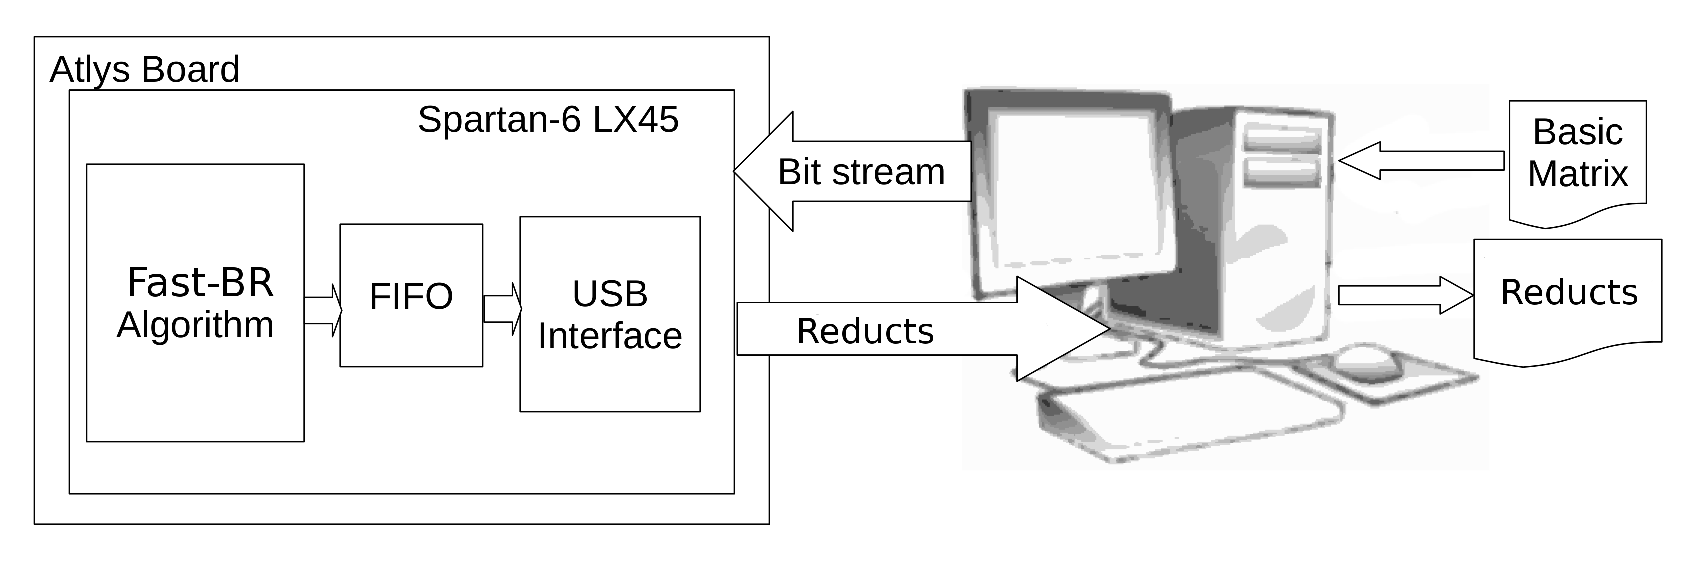
\includegraphics[width=13cm]{Arquitecture_fast-br.eps}
    \end{center}
\caption{Proposed hardware software platform.}
\label{figArq}
\end{figure}

\subsection{Hardware architecture}
\label{sect:4}

\begin{figure}[htb]
    \begin{center}
        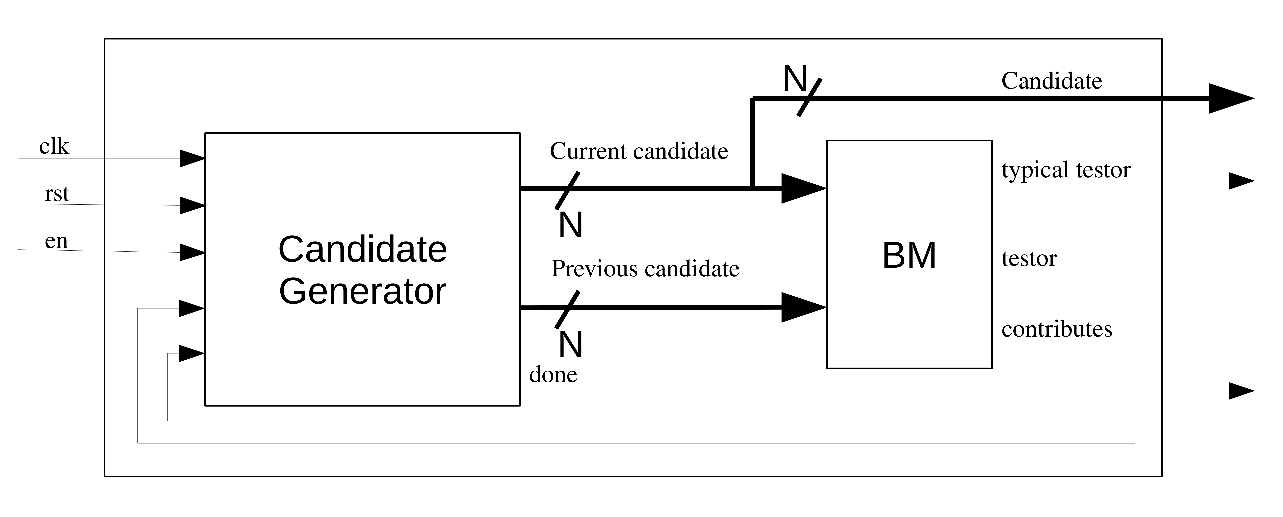
\includegraphics[width=13cm]{CT-ext_arq.eps}
    \end{center}
\caption{Fast-BR Architecture.}
\label{fig:3}
\end{figure}

In the hardware architecture, an attribute subset is handled as an $n$-tuple, using a positional 
representation for all the $n$ attributes of a basic matrix $BM$. Given a subset $T$, its $n$-tuple representation 
has a 1 in the corresponding position $j$ for each $x_j \in T$ and 0 otherwise.
The process of deciding whether an $n$-tuple is a super-reduct of $BM$ involves
comparing the candidate against each one of the $BM$'s rows. For
software-only implementations, this is a big disadvantage, specially for large 
matrices with many rows. The proposed hardware architecture exploits the parallelism 
inherent in the Fast-BR algorithm
and evaluates whether a candidate is a reduct, or not, in a single
clock cycle. The hardware implementation of Fast-BR is composed of two modules, the $BM$ module and the Candidate Generator module, as shown in
Fig.\,\ref{fig:3}. 

The $BM$ module stores the input matrix and
includes all the logic needed to decide whether an $n$-tuple is a super-reduct. The candidate
generator module produces the candidates ($n$-tuples) to be
evaluated by the $BM$ module. In order to calculate the next candidate
according to the Fast-BR algorithm, the architecture feedbacks the
evaluation result of the previous candidate to the generator module;
this drastically reduces the number of candidates tested and
consequently the number of iterations needed by the algorithm. 


\begin{figure}[htb]
    \begin{center}
        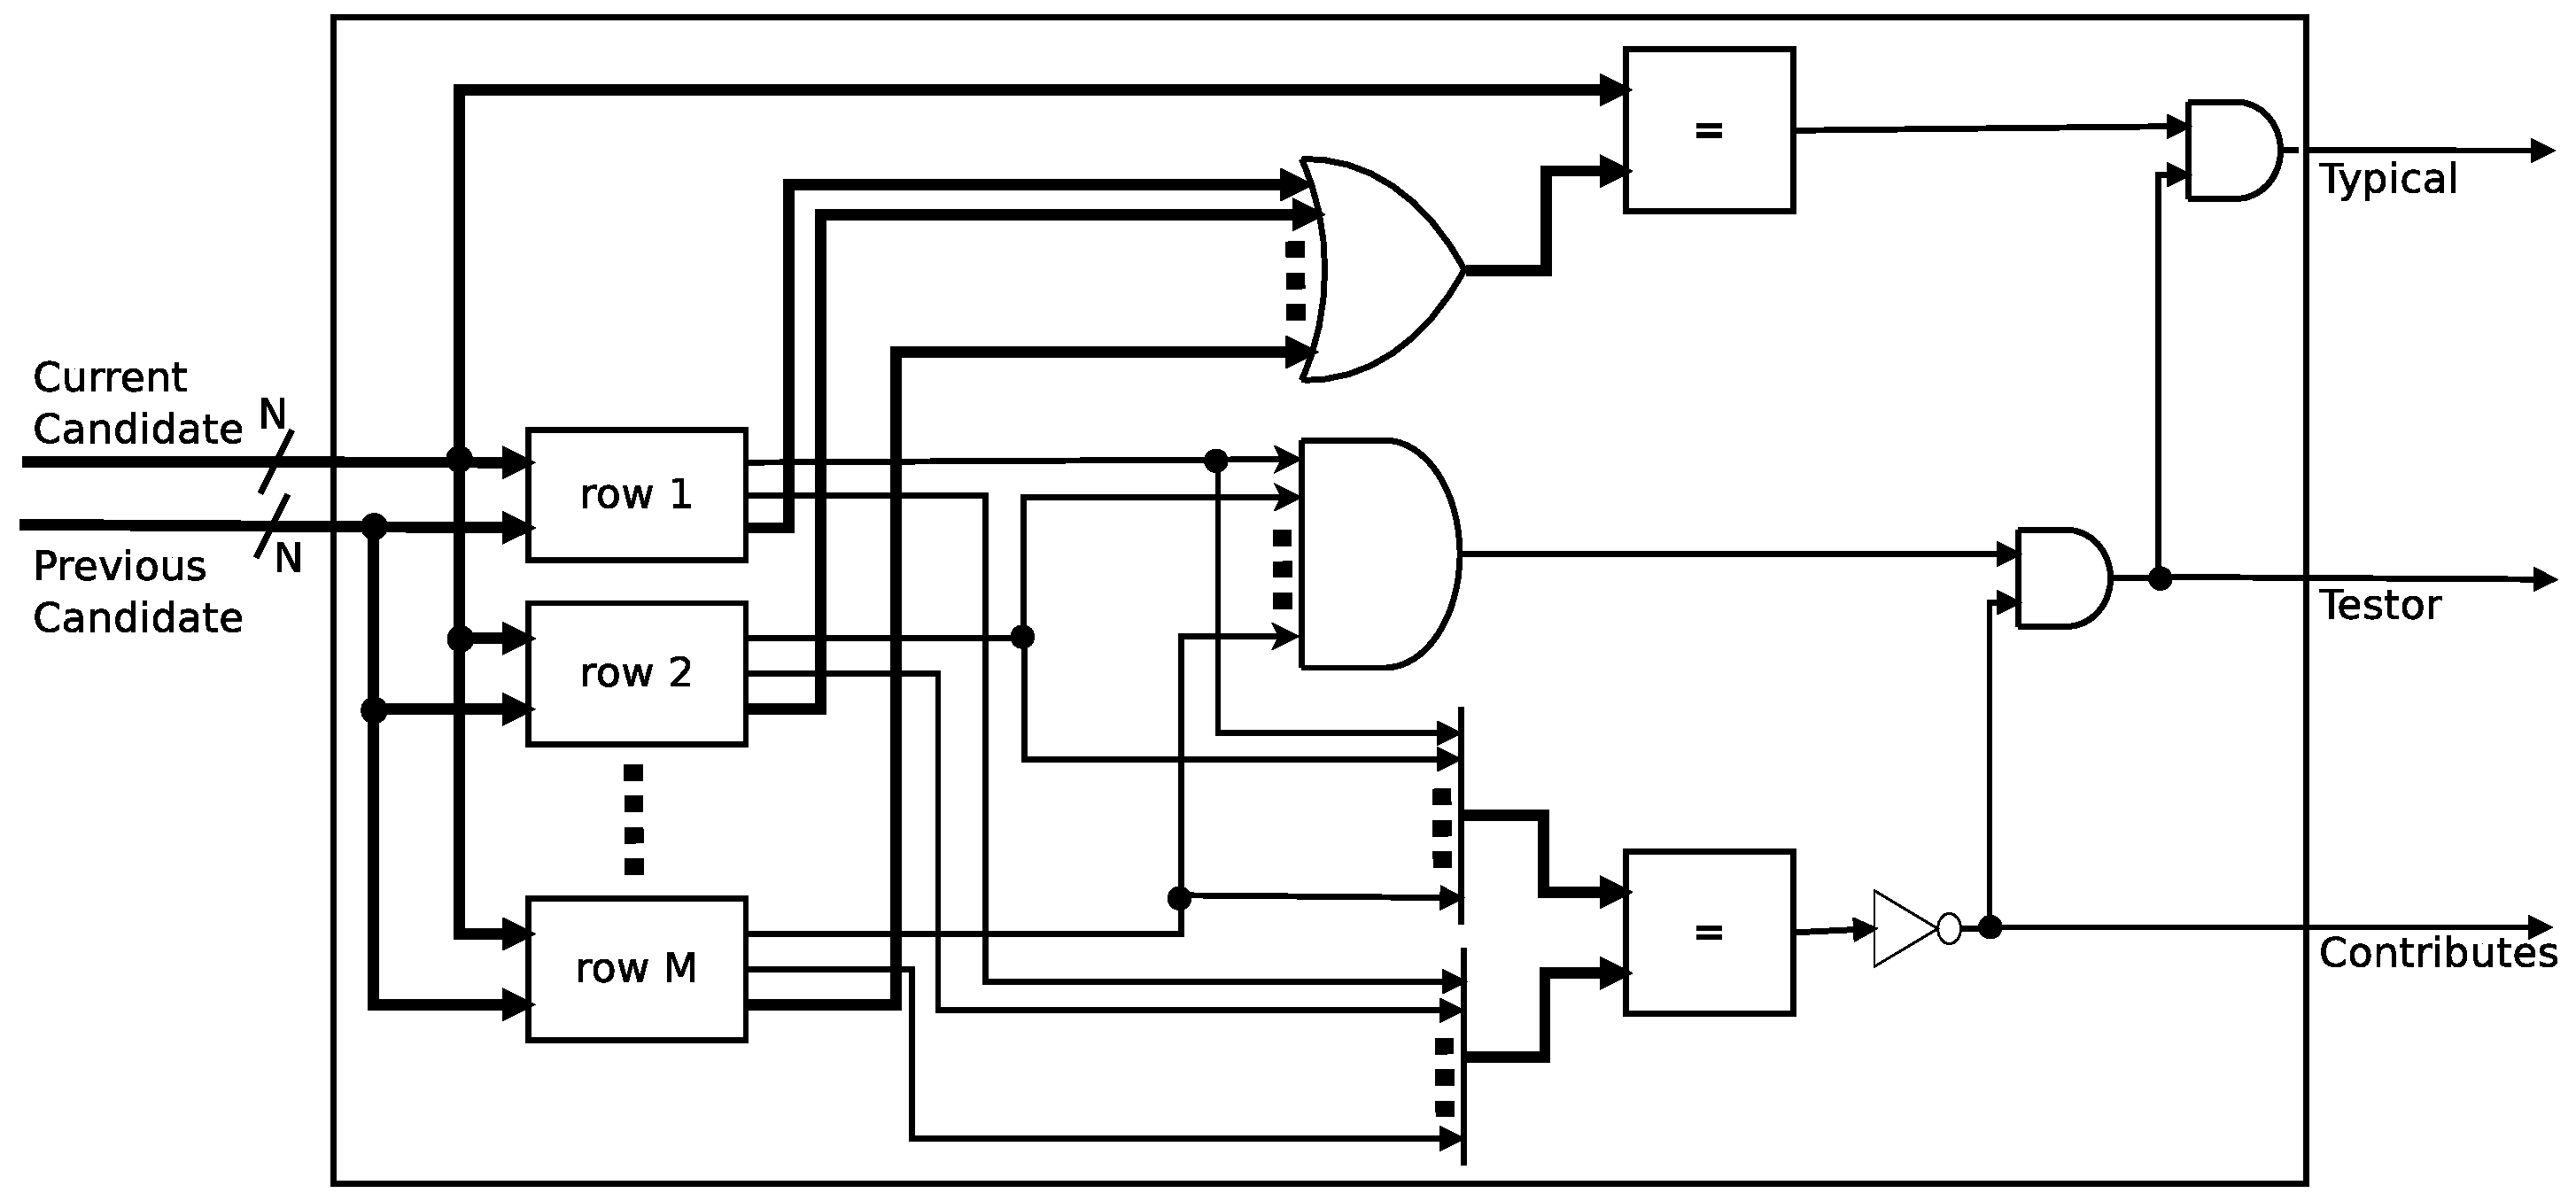
\includegraphics[height=6cm]{BM_module.eps}
    \end{center}
\caption{$BM$ module.}
\label{fig:4}
\end{figure}

The $BM$ module is composed of $M$ sub-modules named \textit{row~i}, as shown
in Fig.\,\ref{fig:4}. Each \textit{row~i} module contains a row ($n$ bits)
of the $BM$ matrix and the logic needed to perform a super-reduct evaluation. To decide
whether an $n$-tuple is a super-reduct, a bitwise AND operation is performed
between the value stored in each \textit{row~i} module and the current
candidate, as shown in Fig.\,\ref{fig:row}. If at least one bit of the AND operation is TRUE,
then the output \textit{Testor} of that particular \textit{row~i} sub-module
will be TRUE. The same operation is performed over the previous candidate.
If the output \textit{Testor} is different from
the output \textit{Contributes} for any \textit{row~i} sub-module,
it means that the current candidate reduces the amount of zero rows regarding the previous candidate and
then, the output \textit{Contributes} from the $BM$ module becomes TRUE.
If the output $Testor$ of all  \textit{row~i} sub-modules is
TRUE, then the output \textit{Testor} of the $BM$ module will be TRUE,
which means that the candidate is a super-reduct of $BM$.


\begin{figure}[htb]
    \begin{center}
        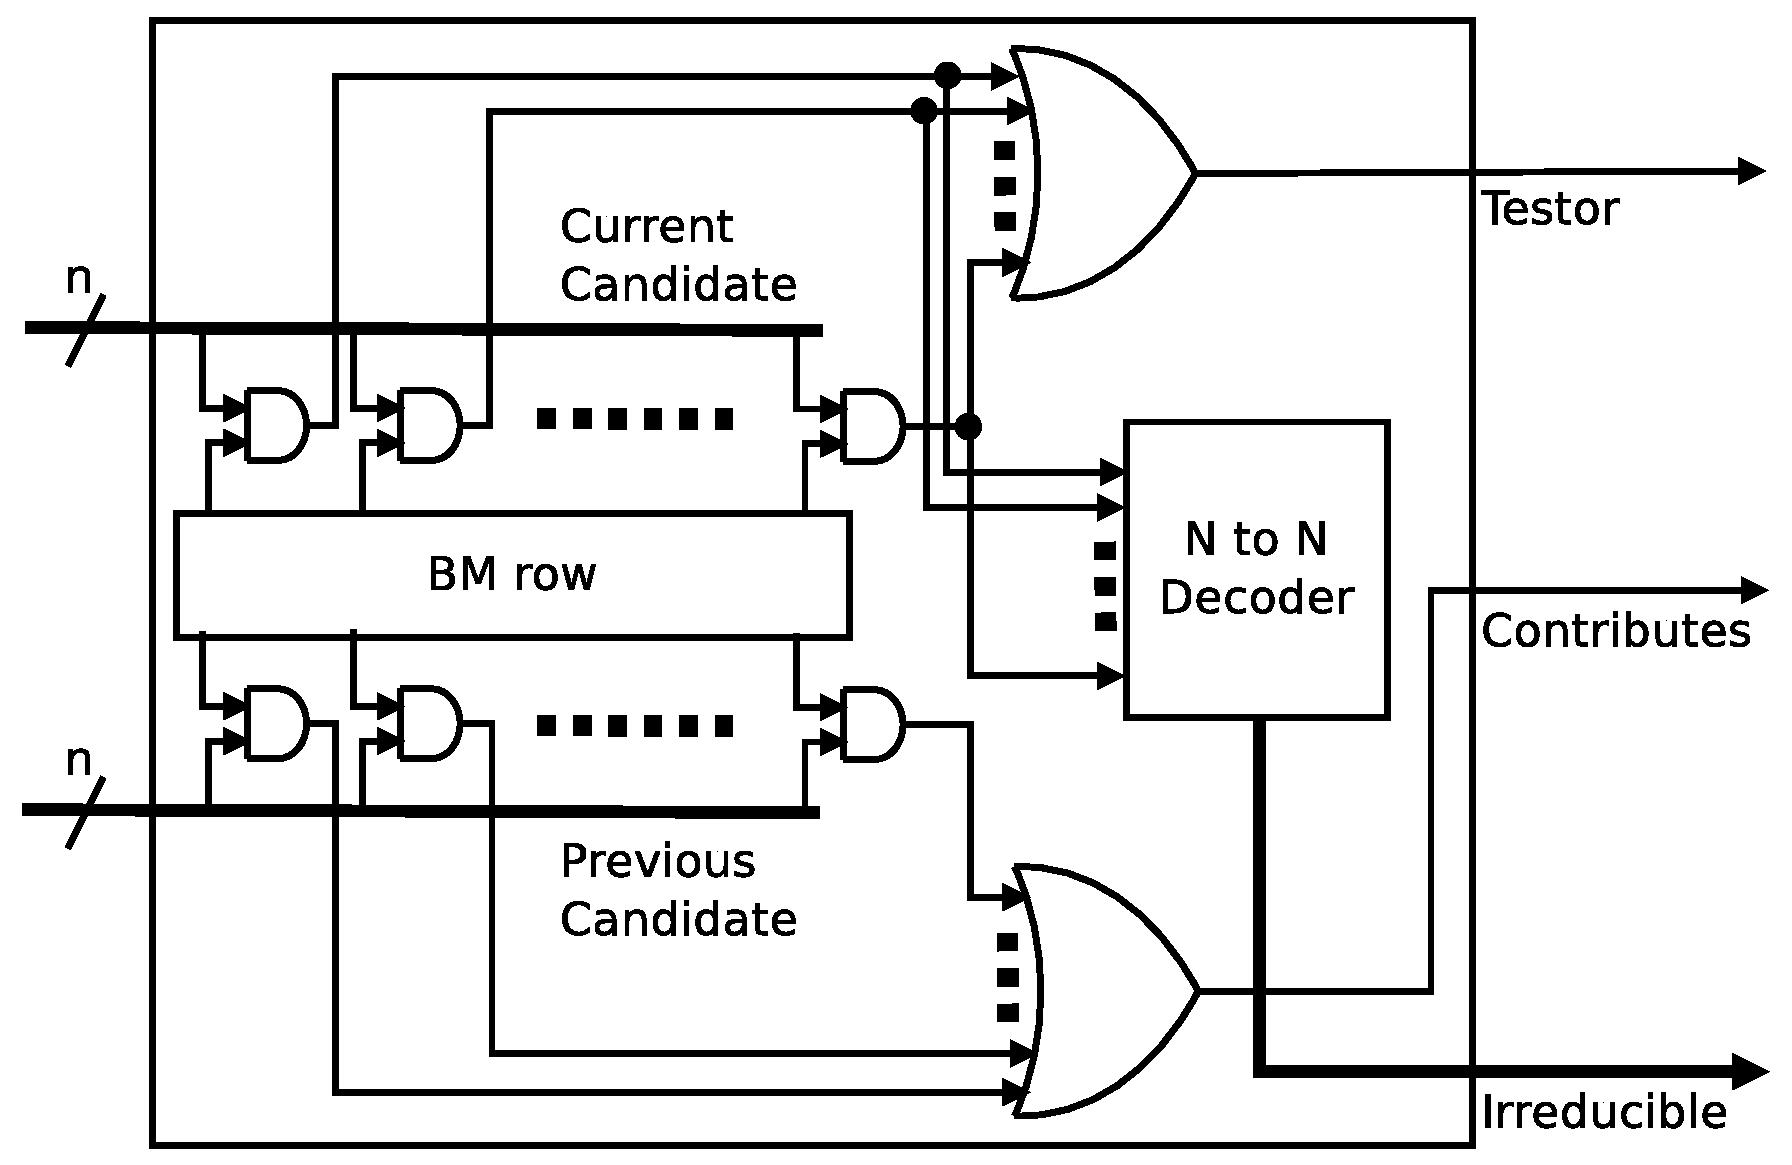
\includegraphics[height=6cm]{BM_row.eps}
    \end{center}
\caption{$BM$ row.}
\label{fig:row}
\end{figure}

In order to verify the irreducible condition, an \textit{N~to~N~Decoder}
receives as input the result of the AND operation between the current candidate and the corresponding $BM$ row.
The output from the \textit{N~to~N~Decoder} repeats the input when there is only one bit set
to 1, and returns zero otherwise. For those rows with only one bit having a 1 after ANDed with the candidate,
the attribute in the position of that bit is indispensable if the candidate is a super-reduct.
According to definition of reduct, every attribute must be indispensable. %This idea is stated in definition~1 of \citep{R13}.

\setlength{\tabcolsep}{3pt}
\begin{table}[!htb]
    \begin{minipage}{.5\linewidth}
      \caption{An example of reduct.}\label{table4}
      \centering
        \begin{tabular}{ ccccc|ccccc }
 			\hline                       
  			\multicolumn{5}{c|}{Cand. $\{x_0, x_1\}$} & 
  			\multicolumn{5}{c}{Decoder output} \\
  			\hline
			  $x_0$ &   $x_3$ &   $x_4$ &   $x_1$ &   $x_2$ &
  			  $x_0$ &   $x_3$ &   $x_4$ &   $x_1$ &   $x_2$ \\
  			\hline
  			1 & 0 & 0 & 0 & 0 & 1 & 0 & 0 & 0 & 0\\
  			0 & 0 & 0 & 1 & 0 & 0 & 0 & 0 & 1 & 0\\
  			1 & 0 & 0 & 1 & 0 & 0 & 0 & 0 & 0 & 0\\
  			\hline  
  			\multicolumn{5}{c|}{Candidate $=$} & 1 & 0 & 0 & 1 & 0\\
  			\hline  
		\end{tabular}
	%\end{table}
	%\begin{table}[!htb]
    \end{minipage}%
    \begin{minipage}{.5\linewidth}
      \centering
        \caption{An example of non reduct.}\label{table5}
        \begin{tabular}{ ccccc|ccccc }
 			\hline                       
  			\multicolumn{5}{c|}{Cand. $\{x_0, x_4\}$} & 
  			\multicolumn{5}{c}{Decoder output} \\
  			\hline
  			%\multicolumn{5}{c|}{$x_0~x_3~x_4~x_1~x_2$}&\multicolumn{5}{c}{$x_0~x_3~x_4~x_1~x_2$}\\
  			  $x_0$ &   $x_3$ &   $x_4$ &   $x_1$ &   $x_2$ &
  			  $x_0$ &   $x_3$ &   $x_4$ &   $x_1$ &   $x_2$ \\
  			\hline
  			1 & 0 & 1 & 0 & 0 & 0 & 0 & 0 & 0 & 0\\
  			0 & 0 & 1 & 0 & 0 & 0 & 0 & 1 & 0 & 0\\
  			1 & 0 & 1 & 0 & 0 & 0 & 0 & 0 & 0 & 0\\
  			\hline  
  			\multicolumn{5}{c|}{Candidate $\neq$} & 0 & 0 & 1 & 0 & 0\\
  			\hline  
		\end{tabular}
    \end{minipage} 
\end{table}

Taking as example the ordered basic matrix of Table~\ref{table2}. In Table~\ref{table4} the irreducibility of  $\{x_0,x_1\}$ is evaluated while the same is done for $\{x_0,x_4\}$ in Table~\ref{table5}. Left rows show the result of the AND operation between each row of $BM$ and the candidate, while those rows in the right show the decoder output taking as input its corresponding left row. In the last row, the result of an OR operation over all above bits is shown. According to our previous explanation, the candidate $\{x_0,x_1\}$ is a reduct given that the result of the OR operation is equal to the candidate itself; while candidate $\{x_0,x_4\}$ is not.

\begin{figure}[t]
    \begin{center}
        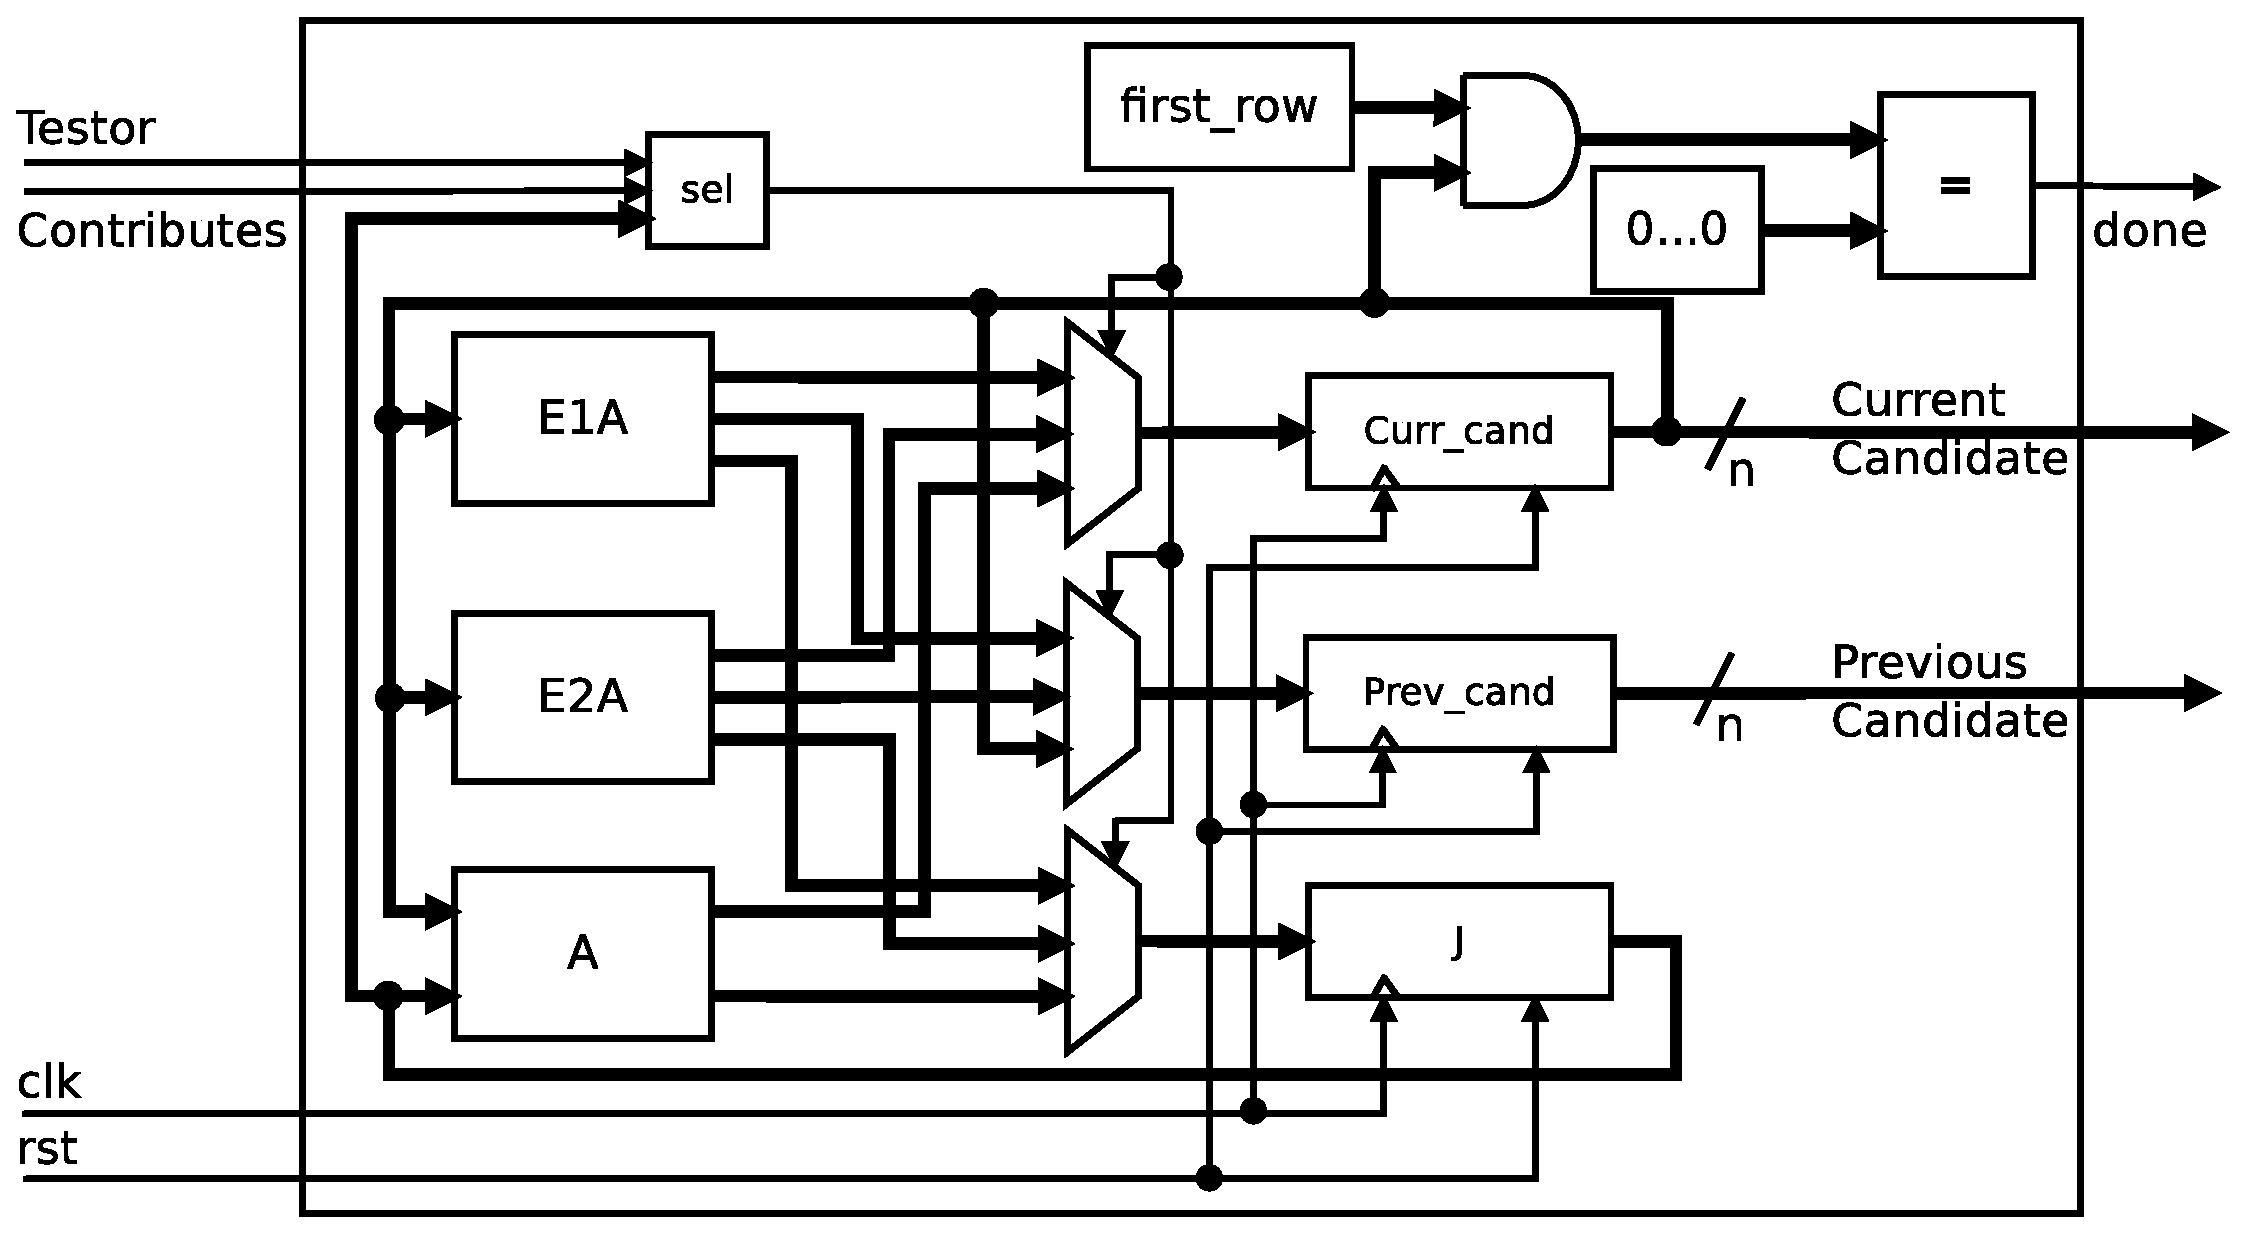
\includegraphics[height=6cm]{CandGen.eps}
    \end{center}
\caption{Candidate Generator module.}
\label{fig:5}
\end{figure}

The candidate generator module (Fig.\,\ref{fig:5}) uses the feedback from the $BM$ module
to calculate the next candidate to be evaluated. The
candidate generator module consists of three
registers for holding the current candidate (\textit{$Curr\_cand$}), the previous candidate
(\textit{$Prev\_cand$}) and the last added attribute ($J$). These registers values are updated
by the modules EA1, EA2 and A.

Depending on the combination of the input values, the outputs E1A,
E2A or A are used for updating the records. Table~\ref{tab_CandGen} shows how the records are updated 
according to the values of \textit{Testor}, \textit{Contributes} and $J$ inputs. 
This operation is computed by the module \textit{sel} shown in Fig.\,\ref{fig:5}.

 \begin{table}[htb]
		\caption{Candidate Generator Selector.} \label{tab_CandGen}
		\centering
 	\begin{tabular}{ccc}
 			\hline
 			Priority & Condition & Registers update\\
 			\hline
 			1 & \multicolumn{1}{>{\centering\arraybackslash}m{1in}}{$J=J_{max}$
 				($J_{max}=$ max value of $J$)} & \multicolumn{1}{>{\centering\arraybackslash}m{2in}}{
 				$Curr\_cand$ $\leftarrow$ E2A
 				$Prev\_cand$~$\leftarrow$~E2A
 				$J$~$\leftarrow$~E2A}\\
 			\hline
 			2 & \multicolumn{1}{>{\centering\arraybackslash}m{1.2in}}{Contributes $=0$ or Testor $=1$} &
 			\multicolumn{1}{>{\centering\arraybackslash}m{2in}}{
 				$Curr\_cand$ $\leftarrow$ E1A
 				$Prev\_cand$~$\leftarrow$~E1A
 				$J$~$\leftarrow$~E1A}\\
 			\hline
 			3 & \multicolumn{1}{>{\centering\arraybackslash}m{1.2in}}{Contributes $=1$ or Testor $=0$}&
 			\multicolumn{1}{>{\centering\arraybackslash}m{2in}}{
 				$Curr\_cand$ $\leftarrow$ A
 				$Prev\_cand$~$\leftarrow$~$Curr\_cand$
 				$J$~$\leftarrow$~A}\\
 			\hline       
 	\end{tabular}             
 \end{table}

The submodule $A$, shown in Fig.\,\ref{fig:subA}, assigns 1 to the next attribute at the right of 
the last bit with value 1 in the input candidate. The outputs of the submodule $A$ are the new candidate 
and $J+1$.

The submodule $E1A$, shown in Fig.\,\ref{fig:subEA1}, comprises the \textit{Rem$\_1$} 
(Fig.\,\ref{fig:subRem1}) and $A$ submodules. 
The submodule \textit{Rem$\_1$} deletes the last attribute added to the input candidate. 
This action is performed by a priority encoder which locates the last bit with value 1 in the input candidate. 
\textit{Rem$\_1$} outputs represent the previous candidate and the index of the deleted bit. 
%: $J$ and \textit{candidate} which is the input candidate without the last attribute. 
These outputs are connected to the corresponding inputs of the
submodule $A$, in order to add an attribute in the corresponding position. Finally, the outputs of $E1A$ 
represent the new candidate to be evaluated, the previous candidate and the index where the new attribute 
was added to the current candidate.

\begin{figure}[htb]
\centering
\begin{minipage}{.5\textwidth}
  \centering
   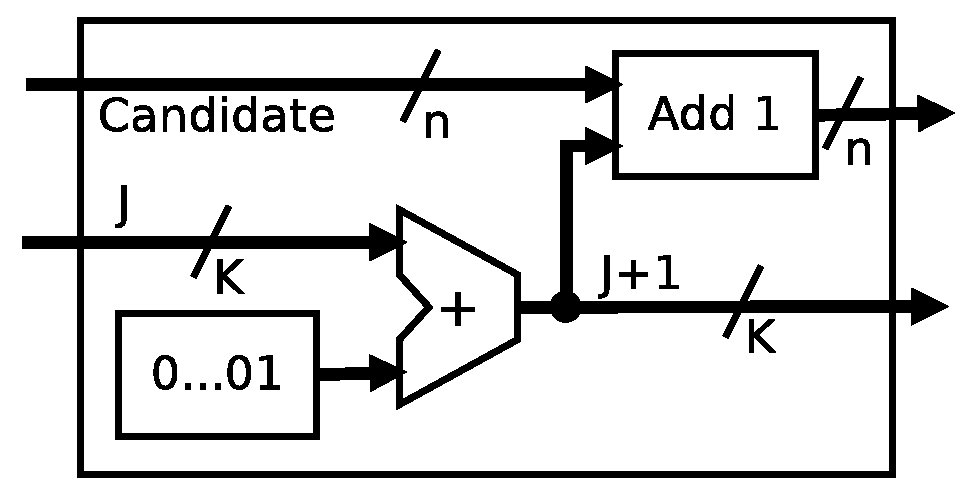
\includegraphics[width=.7\linewidth , height=3cm]{Add1.eps}
  \caption{Submodule A.}
  \label{fig:subA}
\end{minipage}%
\begin{minipage}{.5\textwidth}
  \centering
   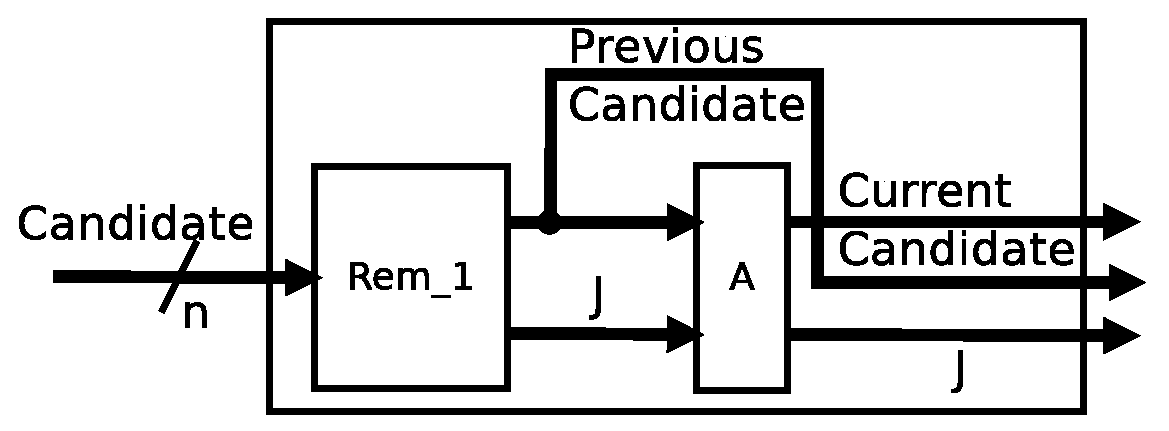
\includegraphics[width=\linewidth , height=3cm]{EA1.eps}
  \caption{Submodule E1A.}
  \label{fig:subEA1}
\end{minipage}
\end{figure}

Finally, the submodule $E2A$ removes the last two attributes from the
input candidate, and then adds the following corresponding attribute. This 
operation is performed by means of two \textit{Rem$\_1$} submodules and an $A$ submodule, as 
shown in Fig.\,\ref{fig:subEA2}.

In order to check if the execution of the Fast-BR  algorithm has finished, the result of an AND 
operation between the current candidate and the first row of the basic matrix is compared to 
the null $n$-tuple ($0,...,0$), as shown in the upper right corner of Fig.\,\ref{fig:5}. If the 
result of this comparison is TRUE, then the output $done$ is activated because any further 
candidate will not satisfy the super-reduct condition over the first row of $BM$.

\begin{figure}[htb]
\centering
\begin{minipage}{.5\textwidth}
  \centering
   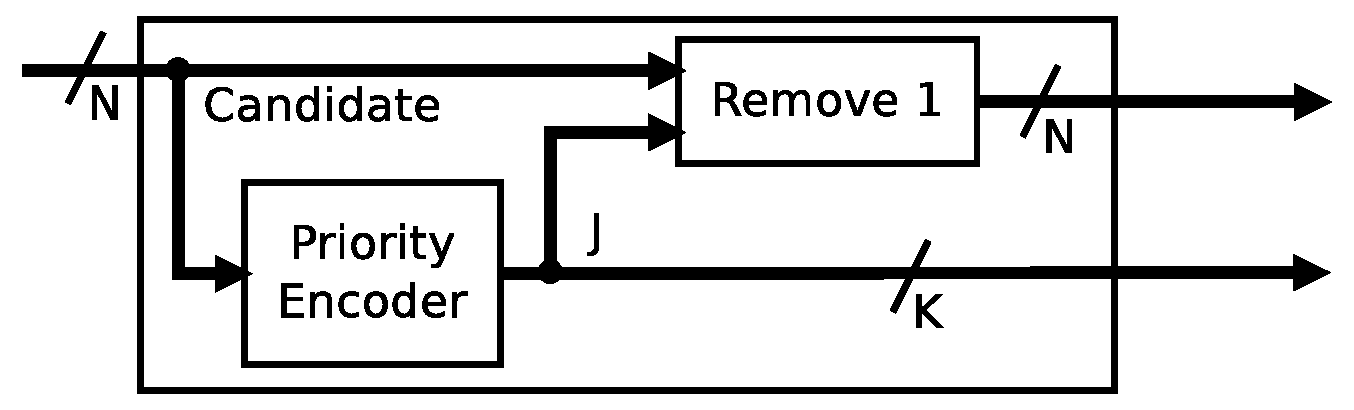
\includegraphics[width=\linewidth , height=3cm]{Rem1.eps}
  \caption{Submodule $Rem\_1$.}
  \label{fig:subRem1}
\end{minipage}%
\begin{minipage}{.5\textwidth}
  \centering
   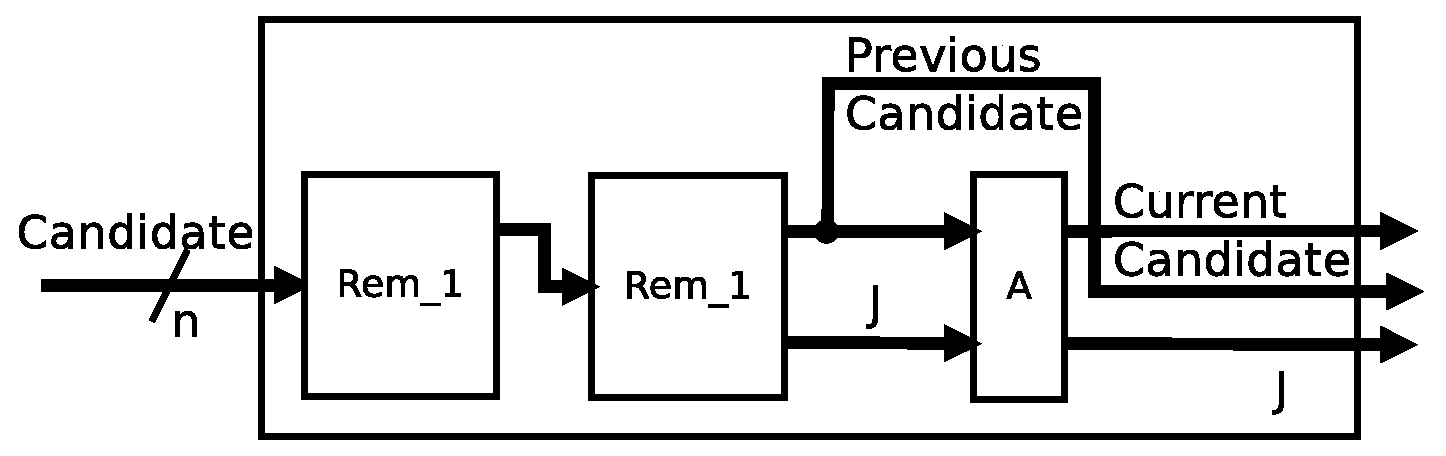
\includegraphics[width=\linewidth , height=3cm]{EA2.eps}
  \caption{Submodule E2A.}
  \label{fig:subEA2}
\end{minipage}
\end{figure}

\subsubsection*{The FPGA-based board}
The Atlys board from Digilent \citep{R15} was selected as the prototyping board. This board is 
a development and prototyping platform based on a Xilinx Spartan-6 LX45 FPGA, speed grade -3. The Atlys board 
supports device programming and simplified user-data transfer at a maximum rate of 48MB/s, over 
a single USB connection. 

The communication between the host PC and the FPGA uses the Digilent Synchronous 
Parallel Interface (DSTM) protocol \citep{R25}. Reducts $n$-tuples, computed by the 
proposed architecture, are buffered within a FIFO in order to be split into bytes. These bytes 
are then buffered into a double clocked FIFO \citep{R26} to be read from the PC. This last FIFO 
ensures the output interface operation at 48MHz, as required by the DSTM protocol.

\subsection{Software Description}
\label{sect:5}

The software component allows the user to provide the basic matrix in a 
plain text file following the format shown in Fig.\,\ref{fig:8}. The software component is responsible for 
programming the FPGA device and communicating with the board during reduct computation.

First, the basic matrix is reorganized by setting one of the rows with the minimum amount of ones as the 
first row and swapping columns in such a way those with a 1 in the first row appear on the left. 

Using the sorted basic matrix, a VHDL file is generated and the synthesis and optimization process is started.
This way, the optimization stage takes advantage of the basic matrix data to minimize the FPGA resource 
utilization. Then, the programming file for the FPGA device is generated.

On the running stage, the software component interacts with the hardware architecture. 
First, the device is programmed with the bit-file obtained from the previous stage. Then, the
hardware architecture starts computing reducts. 
The software component keeps pulling through a USB port for new reducts in the output 
FIFO until the $done$ signal is activated in the FPGA.

As a result of the sorting process, the order of attributes in the basic matrix is altered as can 
be seen comparing Tables~\ref{table1} and~\ref{table2}. Consequently, the reducts calculated 
in the FPGA must be codified according to the order of columns in the original basic matrix. This task 
is performed by the software component and then the results are written to the output file.

\begin{figure}[t]
    \begin{center}
       \includegraphics[height=2.8cm]{infile.eps}
    \end{center}
\caption{Input file format.}
\label{fig:8}
\end{figure}


\section{Conclusions}
\label{sect:8}
In this work, we present the design and implementation of a new hardware software platform for
computing all reducts in a dataset.  Unlike most of the existing hardware 
architectures for feature selection, our proposal computes all the
minimal subsets of attributes that preserve the classification accuracy of the original dataset.
The good performance of our hardware implementation, compared to the software approach, is 
feasible due to the high level of parallelism implicit in the candidate evaluation process of 
the Fast-BR algorithm; which can be efficiently implemented on an FPGA. 
This proposed architecture offers an alternative to previous hardware implementations; being 
faster in most of the cases, by evaluating less candidates to be reducts. 
 

Even though our platform can process larger basic matrices than previous ones, its resource utilization 
determines the maximum size of the basic matrix that can be solved (this is, indeed, the 
main limitation of our proposal), for this reason, the search for new algorithms that could be efficiently implemented on an FPGA constitutes the main direction for future work. Improvements, such as testing two 
or more candidates at the same time, are still unexplored and would be evaluated in further studies.



%\section*{References}
\bibliographystyle{elsarticle-harv}


%% References without bibTeX database:

\begin{thebibliography}{00}

\bibitem[Cheguis et al.(1955)]{Cheguis55}Cheguis, I. A. and Yablonskii, S. V. (1955). Uspieji Matematicheskij Nauk (In Russian).66, 182--184.

\bibitem[Compton et al.(2002)]{R29}Compton, K., and Hauck, S. (2002). Reconfigurable computing: a survey of systems and software. ACM Computing Surveys (csuR), 34(2), 171-210.
\bibitem[Cumplido et al.(2006)]{R10} Cumplido, R., Carrasco, A. and Feregrino, C. (2006). On the Design and Implementation of a High Performance Configurable Architecture for Testor Identification. Lectures Notes on Computer Science, 4225, 665-673.
\bibitem[Djukova(2005)]{R8}Djukova, E. V. (2005). On the number of irreducible coverings of an integer Matrix. Computational Mathematics and Mathematical Physics, 45, 903-908.
\bibitem[Dmitriev et al.(1966)]{R12} Dmitriev, A. N.,  Zhuravlev, Y. I. and Krendeliev, F. P. (1966). About Mathematical Principles of Objects and Phenomena Classification. Diskretni Analiz, 7, 3-17.
\bibitem[G\'omez(2001)]{R16}G\'omez, M. (2001). Hardware-in-the-Loop Simulation. Embedded Systems Programming, 14, 38-49.

\bibitem[Grze et al.(2013)]{Grze13}Grze, T., Kopczynski, M., Stepaniuk, J. (2013). FPGA in Rough Set Based Core and Reduct Computation. In Rough Sets and Knowledge Technology, 263-270.

\bibitem[Guyon et al.(2003)]{R4}Guyon, I. and Elisseeff, A. (2003). An introduction to variable and feature selection. Journal of Machine Learning Research, 3, 1157-1182.
\bibitem[Jain et al.(1997)]{R3}Jain, A. and Zongker, D. (1997). Feature Selection: Evaluation, Application, and Small Sample Performance. IEEE Transactions on Pattern Analysis and Machine Intelligence, 9, 153-158.

\bibitem[Jensen and Shen (2014)]{Jensen14}Jensen, R., Tuson, A., Shen, Q. (2014). Finding rough and fuzzy-rough set reducts with SAT. Information Sciences, 255, 100-120.

\bibitem[Kopczynski et al.(2014)]{Kop14}Kopczynski, M., Grze, T., Stepaniuk, J. (2014). FPGA in Rough-Granular Computing : Reduct Generation. In 2014 IEEE/WIC/ACM International Joint Conferences on Web Intelligence (WI) and Intelligent Agent Technologies (IAT), 364-370. 

\bibitem[Kudryavtsev(2006)]{R9}Kudryavtsev, V. B. (2006). Test recognition theory. Discrete Applied Mathematics, 16, 319-350.
\bibitem[Lazo-Cort\'es et al.(1995)]{R32}Lazo-Cort\'es, M., Ruiz-shulcloper, J. (1995). Determining the feature relevance for non-classically described objects and a new algorithm to compute typical fuzzy testors. Pattern Recognition Letters, 16(12), 1259-1265.
\bibitem[Lazo-Cort\'es et al.(2001)]{R1}Lazo-Cort\'es, M., Ruiz-shulcloper, J., and Alba-cabrera, E. (2001). An Overview of the Evolution of the Concept of Testor. Pattern Recognition, 34, 753-762.

\bibitem[Lazo-Cort\'es et al.(2015)]{Lazo15}Lazo-Cortés, M. S., Mart\'inez-Trinidad, J. F., Carrasco-Ochoa, J. A. and S\'anchez-D\'iaz, G. (2015). On the relation between rough set reducts and typical testors. Information Sciences, 294, 152-163.

\bibitem[Lias-Rodr\'{\i}guez et al.(2013)]{Lias13}Lias-Rodr\'{\i}guez, Alexsey and S\'{a}nchez-D\'{\i}az, Guillermo. (2013). An Algorithm for Computing Typical Testors Based on Elimination of Gaps and Reduction of Columns. International Journal of Pattern Recognition and Artificial Intelligence, 27, 1350022.

\bibitem[Mart\'inez et al.(2007)]{Mart07}Mart\'inez, N., Le\'on, M. and Garc\'ia, Z. (2007). Features selection through FS-testors in case-based systems of teaching-learning. In MICAI 2007: Advances in Artificial Intelligence, 1206-1217.

\bibitem[Mart\'inez-Trinidad et al.(2001)]{R5}Mart\'inez-Trinidad, J.F. and Guzm\'an-Arenas, A. (2001). The Logical Combinatorial Approach to Pattern Recognition an Overview through Selected Works. Pattern Recognition, 34, 741-751.
	
\bibitem[Medina et al.(2007)]{Med07}Medina, D., Mart\'inez, N., Garc\'ia, Z., Ch\'avez, M. and Garc\'ia, M. (2007). Putting Artificial Intelligence Techniques into a Concept Map to Build Educational Tools. In Nature Inspired Problem-Solving Methods in Knowledge Engineering, 617-627.

\bibitem[Mukamakuza et al.(2014)]{Mukamakuza2014}Mukamakuza, Carine Pierrette and Wang, Jiayang. (2014). Dynamic Reducts Computation Analysis Based on Rough Sets. Natural Computation (ICNC), 2014 10th International Conference on. 480--485.

\bibitem[Parthal\'{a}in et al.(2008)]{Parthalain08}Parthal\'{a}in, Neil Mac and Jensen, Richard and Shen, Qiang. (2008). Finding fuzzy-rough reducts with fuzzy entropy. IEEE International Conference on Fuzzy Systems. 1282--1288.

\bibitem[Pawlak (1981)]{Pawlak81} Pawlak, Zdislaw. (1981). Classification of objects by means of attributes. Polish Academy of Sciences [PAS]. Institute of Computer Science.

\bibitem[Piza-Davila et al.(2015)]{Piza13}Piza-Davila, I., S\'anchez-D\'iaz, G., Aguirre-Salado, C. A., Lazo-Cortes, M. S. (2015). A parallel hill-climbing algorithm to generate a subset of irreducible testors. Applied Intelligence, 42(4), 622-641.

\bibitem[Pocek et al.(2013)]{R30}Pocek, K., Tessier, R. and DeHon, A. (2013). Birth and adolescence of reconfigurable computing: A survey of the first 20 years of field-programmable custom computing machines. In Highlights of the First Twenty Years of the IEEE International Symposium on Field-Programmable Custom Computing Machines (pp. 3-19).

\bibitem[Ro\-dr\'iguez et al.(2014)]{Rod14} Rodr\'iguez, V., Mart\'inez, J. F., Carrasco, J. A., Lazo, M. S., Cumplido, R. and Feregrino-Uribe, C. (2014). A hardware architecture for filtering irreducible testors. In ReConFigurable Computing and FPGAs (ReConFig), 2014 International Conference on, 1-4.

\bibitem[Rojas et al.(2007)]{R11}Rojas, A., Cumplido, R., Carrasco-Ochoa, J. A., Feregrino, C. and Mart\'inez-Trinidad, J. f. (2007). FPGA Based Architecture for Computing Testors. Lectures Notes on Computer Science, 4881, 188-197.
\bibitem[Rojas et al.(2012)]{R21}Rojas, A., Cumplido, R., Carrasco-Ochoa, J. A., Feregrino, C. and Mart\'inez-Trinidad, J. f. (2012). Hardware-software platform for computing irreducible testors. Expert Systems with Applications, 39, 2203 - 2210.
\bibitem[Ruiz-Shulcloper et al.(1985)]{R31}Ruiz-Shulcloper, J., Aguila-Feros, L. and Bravo-Mart\'inez, A. (1985). BT and TB algorithms for computing all irreducible testors. Revista Ciencias Matem\'aticas, 2, 11-18.
\bibitem[Ruiz-Shulcloper(2008)]{R27}Ruiz-Shulcloper, J. (2008). Pattern recognition with mixed and incomplete data. Pattern Recognition and Image Analysis, 18(4), 563-576.
\bibitem[S\'anchez-D\'iaz et al.(2002)]{R13}S\'anchez-D\'iaz, G. and Lazo-Cort\'es, M. (2002). Modifying BT Algorithm for Improving its Runtimes. Revista Ciencias Matem\'aticas, 20, 129-136.
\bibitem[S\'anchez-D\'iaz et al.(2007)]{R22}S\'anchez-D\'iaz, G. and Lazo-Cort\'es, M. (2007). Fast-BR: An Algorithm for Computing Typical Testor Set. Lecture Notes in Computer Science, 4756, 506-514.
\bibitem[S\'anchez-D\'iaz et al.(2010)]{R23}S\'anchez-D\'iaz, G., Piza-Davila, I, Lazo-Cort\'es, M, 
Mora-Gonz\'alez, M and Salinas-Luna, J. (2010). A Fast Implementation of the Fast-BR Algorithm for the Testor Property Identification. Lecture Notes in Computer Science, 6438, 92-103.
\bibitem[Skowron et al.(1992)]{R40}Skowron, A and Rauszer, C. (1992). The discernibility matrices and functions in information systems. Handbook of Applications and Advances of the Rough Sets Theory, 331-362.

\bibitem[Tiwari et al.(2013)]{Tiwari13}Tiwari, K., Kothari, A., Shah, R. (2013). FPGA Implementation of a Reduct Generation Algorithm based on Rough Set Theory. International Journal of Advanced Electrical and Electronics Engineering (IJAEEE), 2(6), 55-61.

\bibitem[Tiwari and Kothari (2014)]{Tiwari14} Tiwari, K., Kothari, A. (2014). Design and Implementation of Rough Set Algorithms on FPGA : A Survey, 3(9), 14-23.

\bibitem[Torres et al.(2014)]{Torr14}Torres, M., Torres, A., Cuellar, F., Torres, M., Ponce de Le\'on, E. and Pinales, F. (2014). Evolutionary computation in the identification of risk factors. Case of TRALI. Expert Systems with Applications, 41(3), 831-840.

\bibitem[Yahia et al.(2000)]{Yah00}Yahia, M. E., Mahmod, R., Sulaiman, N. and Ahmad, F. (2000). Rough neural expert systems. Expert Systems with Applications, 18(2), 87-99.

\bibitem[Digilent(2013)]{R15}Atlys Board Reference Manual. Digilent, Inc.
\bibitem[Digilent(2010)]{R25}Digilent Synchronous Parallel Interface (DSTM) Programmer's Reference Manual. Digilent, Inc.
\bibitem[Xilinx(2012)]{R26}LogiCORE IP FIFO Generator v9.2. Xilinx Inc.

\bibitem[Xu et al.(2013)]{Xu2013}Xu, Bingxin and Chen, Huiping and Zhu, William and Zhu, Xiaozhong. (2013). Multi-objective cost-sensitive attribute reduction. Proceedings of the 2013 Joint IFSA World Congress and NAFIPS Annual Meeting, IFSA/NAFIPS. 1377-1381.

\end{thebibliography}

\end{document}